 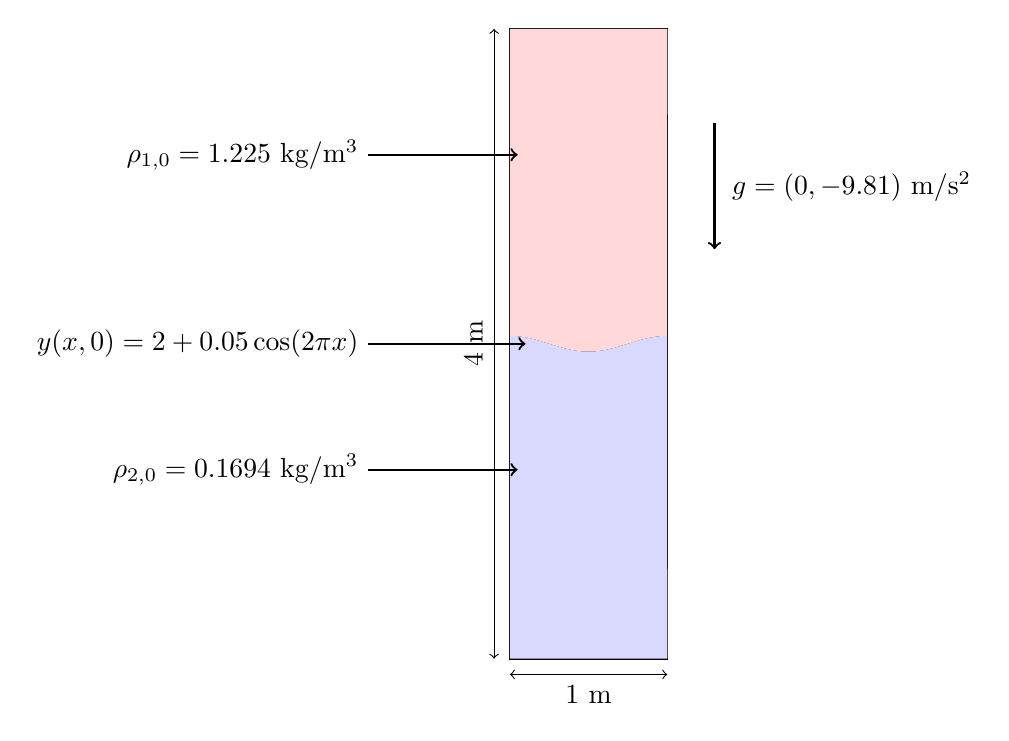
\begin{tikzpicture}[scale=2]

        %=====================
        % Domain
        %=====================
        \draw[thick] (0,0) rectangle (1,4);

        %=====================
        % Interface
        %=====================
        \draw[thick,domain=0:1,samples=200]
        plot (\x,{2 + 0.05*cos(2*pi*\x r)});

        %=====================
        % Fill regions
        %=====================
        \fill[blue!15,domain=0:1,samples=200]
        (0,0)
        -- plot (\x,{2 + 0.05*cos(2*pi*\x r)})
        -- (1,0) -- cycle;

        \fill[red!15,domain=0:1,samples=200]
        (0,4)
        -- plot (\x,{2 + 0.05*cos(2*pi*\x r)})
        -- (1,4) -- cycle;

        %=====================
        % Left-side annotations (densities & interface)
        %=====================

        % Upper fluid density
        \draw[->,thick] (-0.9,3.2) -- (0.05,3.2);
        \node[left,align=right] at (-0.9,3.2)
        {$\rho_{1,0}=1.225~\mathrm{kg/m^3}$};

        % Lower fluid density
        \draw[->,thick] (-0.9,1.2) -- (0.05,1.2);
        \node[left,align=right] at (-0.9,1.2)
        {$\rho_{2,0}=0.1694~\mathrm{kg/m^3}$};

        % Interface function
        \draw[->,thick] (-0.9,2.0) -- (0.1,2.0);
        \node[left,align=right] at (-0.9,2.0)
        {$y(x,0)=2+0.05\cos(2\pi x)$};

        %=====================
        % Gravity annotation (right side)
        %=====================
        \draw[->,thick] (1.3,3.4) -- (1.3,2.6);
        \node[right,align=left] at (1.35,3.0)
        {$\bm g=(0,-9.81)\ \mathrm{m/s^2}$};

        %=====================
        % Dimensions
        %=====================
        \draw[<->] (0,-0.1) -- (1,-0.1);
        \node at (0.5,-0.23) {$1~\mathrm{m}$};

        \draw[<->] (-0.1,0) -- (-0.1,4);
        \node[rotate=90] at (-0.23,2) {$4~\mathrm{m}$};

        %=====================
        % Boundary condition note
        %=====================
        % \node at (0.5,4.25) {Free-slip boundaries};

    \end{tikzpicture}